\chapter{Background}

%\textit{Note: Describe each proven technology / concept shortly that is important to understand your thesis. Point out why it is interesting for your thesis. Make sure to incorporate references to important literature here.}

Although the context of our case study is software engineering, and more specifically in the management of remote agile teams,  the motivation originates from the discipline of psychology.  The psychological process of finding reasons behind a behaviour happens naturally and often unawarely. In the early attempts of studying attribution, Heider \cite{Heider1958} even considers people naive psychologists, who try to make sense of the causes and effects of various happenings. Therefore, this chapter dives deeper into the research surrounding attribution, as it is the phenomenon igniting this thesis. 

The following section presents the reader with the trajectory of the research surrounding attributions.  After elaboration on the \textit{\nameref{PsychologicalBackground}},  we will continue with the circumstances in which this thesis takes place, with a focus on team virtuality and management of software engineering projects.   


\section{Psychological Background} \label{PsychologicalBackground}

\textit{Attribution} is not only the first word in the title of this thesis; it also constitutes the core subject under study. As human beings, we are forming attributions everytime we ask "why" and try to find an answer that argues the cause of an event. The theory that is concerned with studying attributions is known as \textit{Attribution theory} and can be best described through the following definition: 

\begin{quote}
"Attribution theory deals with how the social perceiver uses information to arrive at causal explanations for events. It examines what information is gathered and how it is combined to form a causal judgement". \cite{Fiske1991}
\end{quote}

There are various streams of research that have emerged.  We want to focus on one of the most substantial works in attribution theory, Heider's \textit{The psychology of interpersonal relations}. The work considers the cause of a behaviour to be either internal (e.g., a disposition or a characteristic of a person) or external (e.g. an environmental factor). These are often referred to also as dispositional and situational attribution. 

One of the major areas of interest in the attribution literature concerns the cognitive processes that lead from observation of behaviour to dispositional attribution \cite{Trope1989}. Trope even constructed a two-stage attribution model. This model fundamentally indicates that dispositional attribution is positively related to the identification of the corresponding behaviour and negatively related to the identification of the corresponding situational inducements \cite{Trope1986}. A simplified version of the two-stage modelled is depicted in Figure \ref{fig:twoStageModel}.

\begin{figure}
  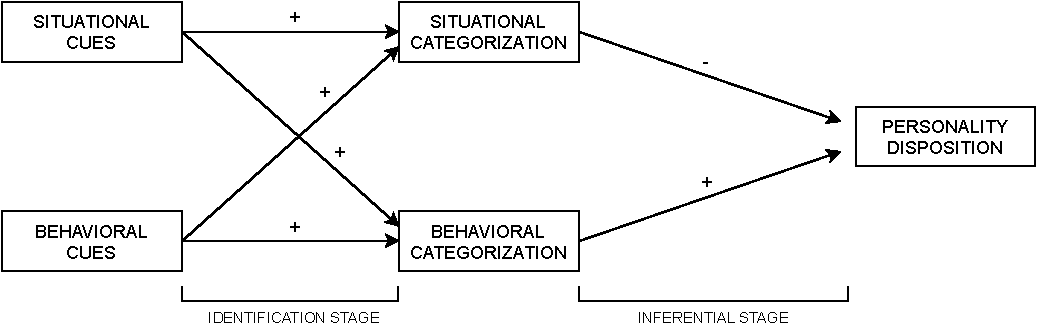
\includegraphics[width=\linewidth]{figures/TwoStageModel.pdf}
  \caption{Two-stage model according to Trope \cite{Trope1986}}
  \label{fig:twoStageModel}
\end{figure}

Another stream of research is concerned with the context in which attributions are formed.  In 1965, social psychologists Edward E. Jones and Keith Davis proposed an explanation for patterns of attribution termed correspondent inference theory \cite{Jones1965}. The basis for the inference is a correspondence between behaviour and disposition, according to the perceiver. They explained that certain conditions make us more likely to make a correspondent inference about someone's behaviour. Following points summarize the conditions proposed by \cite{Jones1965}:

\begin{itemize}
\item Choice: If a behaviour is freely chosen it is believed to be due to internal (dispositional) factors.
\item Accidental vs.  Intentional Behaviour: Behaviour that is intentional is likely to be attributed to the person’s personality, and behaviour which is accidental is likely to be attributed to situation / external causes.
\item Social Desirability: Behaviours low in sociable desirability (non-conforming) lead us to make (internal) dispositional inferences more than socially desirable behaviours.  For example, if you observe a person getting on a bus and sitting on the floor instead of one of the seats, one you interpret this behaviour as non-conforming. This behaviour has low social desirability and is likely to correspond with the personality of the individual.
\item Hedonistic Relevance: If the other person's behaviour appears to directly benefit or harm us,  the attributions we form are also affected. There is a tendency to create more dispositional attributions,  if future events are linked to that person and the dependence is higher.  An example would be a manager's dependency from the subordinates deliverables.
\item Personalism: If the other person's behaviour appears to be intended to have an impact on us, we assume that it is "personal", and not just a by-product of the situation we are both in, which applies more to Hedonistic Relevance.
\end{itemize}

% https://en.wikipedia.org/wiki/Correspondent_inference_theory
% https://www.simplypsychology.org/attribution-theory.html

% Other important work on attribution include covariance theory, https://en.wikipedia.org/wiki/Attribution_bias

Harold Kelley is another researcher who focused on how individuals determine the cause of a behaviour or event.  In his research, he considered information regarding the consensus, consistency,  and distinctiveness of the behaviour or event. Kelley’s model explores these three dimensions and argues they covariate with the person's tendency  to locate the causality \cite{Kelley1967}. 

Another model is proposed by Weiner and colleagues, who focused on the consequences of four different types of causal judgments that people make for events
regarding their performance \cite{Weiner1972}. Specifically, they argued that an individual's expectations, emotions, and behaviours could be predicted by understanding whether the event's cause was believed to be (1) internal or external, (2) stable or unstable, (3) controllable or uncontrollable, and (4) global or specific.  These two models are important because the dimensions described by Kelley illuminate the types of information people use to make attributions, whereas the dimensions identified by Weiner help predict both behavioural and emotional responses. %https://www.researchgate.net/profile/Marion-Eberly/publication/259481760_Beyond_Internal_and_External_A_Dyadic_Theory_of_Relational_Attributions/links/00b4952c1c1e104f5d000000/Beyond-Internal-and-External-A-Dyadic-Theory-of-Relational-Attributions.pdf

Before even taking in consideration behaviours,  Asch’s seminal research on impression formation established that particular “central” personality traits shape the interpretation of subsequent traits and,  the overall impression formed \cite{Asch1961}.  In other words, the first impression we created on someone plays a role in the perception of their future behaviours.

\begin{figure}
  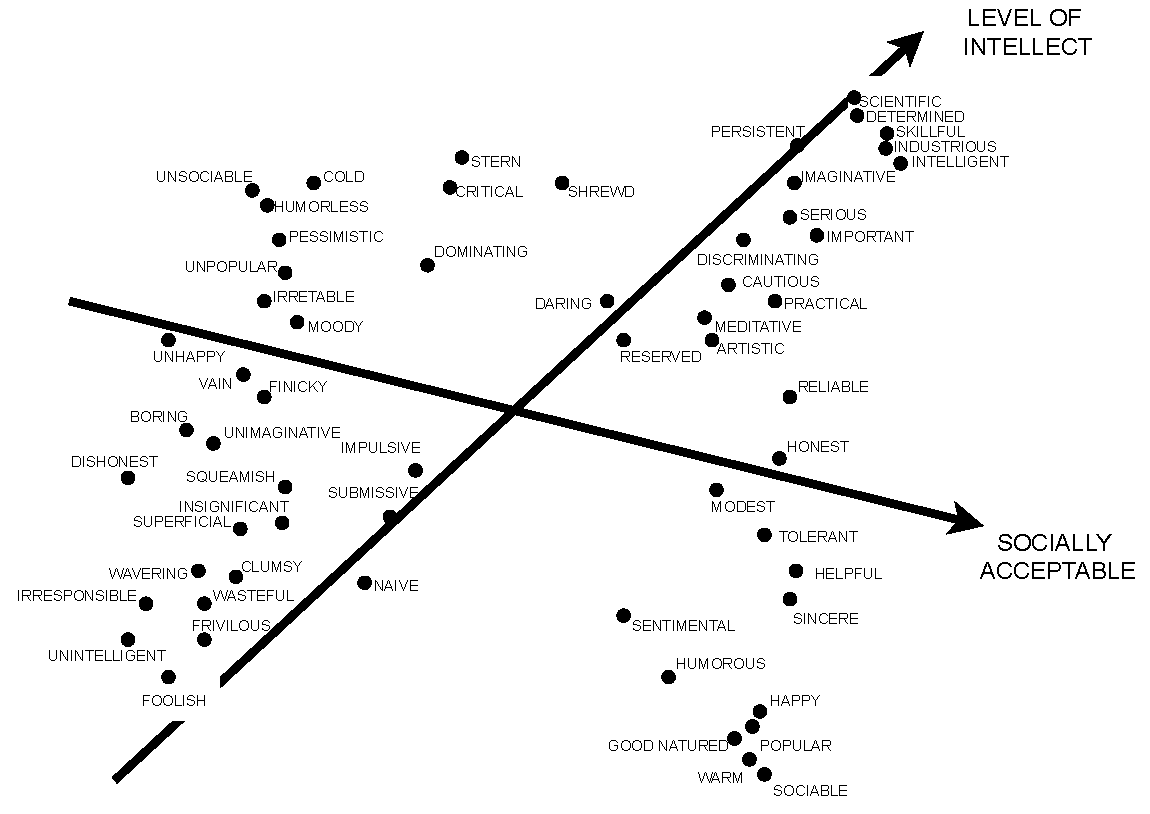
\includegraphics[width=\linewidth]{figures/TwoDimensionsOfAttributions.pdf}
  \caption{Two-dimensional configuration of 60 traits by \cite{Rosenberg1968}}
  \label{fig:twoDimensions}
\end{figure}

Researches have also examined the domains of such perceptions.  Personality judgements are made upon a limited number of domains,  and early studies consider social and intellectual desirability, as the two axes of attribution forming \cite{Rosenberg1968}.

~\autoref{fig:twoDimensions} represents the categorization of 60 distinct attributions.  The labels of these two dimensions have varied over time and the newest research labels them as competence and warmth \cite{Fiske2007, Judd2005}. Warmth is anchored by positive traits such as warm, honest and negative traits such as cold, unreliable and competence is anchored by positive traits such as competent and assertive and negative traits such as inefficient, passive.  For the warmth - cold dimension we use the concept of \textit{social acceptance}, and we treat competence as \textit{level of intellect}. These attributions are presented to illustrate the range of attributions a person can form on another.

Whereas people can make relatively logical assessments of cause and responsibility, as Heider predicted \cite{Heider1958}, researchers have found there are often systematic biases in how we make attributions \cite{Ross1977}. Perhaps the most well known bias is the fundamental attribution error, which is our tendency to make more internal attributions than external attributions for others' behaviours. 

An explanation of the fundamental attribution error can be either of internal or external origin.  Internal explanations have been framed in terms of individuals' perceptual and cognitive information-processing biases \cite{Kelley1980}. An external explanation, which emphasizes that social pressures from the environment are applied to the individual.  Reviews by \cite{Zuckerman1979} of the research on
attributions for success and failure show that, consistent with these assumptions, attributions for success are usually relatively internal and attributions
for failure are usually relatively external. 

Attempts have been made to study the consequences of attribution,  but the results have been ambiguous to interpret the casual link between an attribution and the reaction \cite{Kelley1980}.  Regardless of the research, the hypothesis and results may be revisited to gain more interesting and accurate findings.  \cite{Ickes1976} proposed an attributional analysis of helping behaviour. They hypothesized that more help is given to persons whose need is attributed to unintentional factors rather than intentional ones. \cite{Phares1957} found that when subjects were told that their success on a
judgment task was due to skill, expectancy of future success was higher than
when success was due to chance. On the other hand, failure due to chance
rather than skill yielded higher expectancy of future success.  

Errors in regards to attributions are also regarded from another perspective. This perspective is based on the assumption that attributions have personal implications for the attribution maker. The self-serving attributional bias is exhibited when attributing success internally and failure externally \cite{Duval2002}.  This bias even appears for many psychologists to have achieved the status of an empirical fact \cite{Brown1991} as researchers indeed find a consistent tendency for individuals to attribute success to self \cite{Miller1975}.

Whether an action is attributed to the a person's dispositions or to some aspect of the
environment affects such things as liking the person,  trusting in them,  and their
persuasiveness \cite{Kelley1980}. The externally justified action that harms or frustrates a person is better tolerated and less reciprocated than a similar action attributed to the character of the actor.  Another stream of research looks into the "forgiveness" or tolerability of inappropriate behaviours. The extent to which excused transgressive behaviours are forgiven depends on several factors, such as the perceived match between excuse and transgression \cite{Kim2006}, the sincerity with which the excuse was offered \cite{Zechmeister2004},  how severe the outcome was \cite{Bennett1994},  as well as the time at which the excuse was offered \cite{Frantz2005}.

Considering the objectives of this thesis, our main goal lies not in measuring the fundamental attribution error directly, but rather in investigating the context of dispositional attribution. A focus on the fundamental attribution error would require the employment of techniques of experimental social psychology. More realistically, we want to investigate whether a tendency to attribute dispositions exists. Nonetheless, studies around the fundamental attribution error are taken in consideration, as they contain relevant approaches and knowledge that could be of use when conducting the research for this thesis.  In a world in which the external environment rapidly changes, dispositional attributions might or might not change as well. 

\section{Virtual leadership of software engineering teams} \label{VirtualLeadership}

The pandemic of COVID-19 and the distancing measures in action to prevent its spread, have made digital transformation obligatory for a multitude of businesses and sectors \cite{Fletcher2020}.  Although professionals in most critical roles (such as medical staff) continued to work on a daily basis,  a large part of the working population had to and still works in their home offices (as per submission date of this thesis).  At a first glance this may be a comfortable situation for many compared to the struggles of front-line workers,  but working or studying from home is not without its challenges.  

As subject to this thesis,  we will be looking particularly at the field of software engineering and development.  Software development has never been more relevant, given our digital age and the fact that human experiences and professional and social exchanges often exclusively rely on digital technologies \cite{Yoo2010}.  

Although software development includes activities that can be performed in a distributed setting, switching completely to virtual collaboration and turning private environments of home into offices presented personal and professional challenges.  The teams following agile software development methodologies might be specifically subject to these challenges. According to the agile manifesto,  individuals and interactions are valued over processes and tools,  and customer collaboration over contract negotiation.  These statements depict humans as of great importance in the success of developing software.

The virtuality of teams is a phenomenon dating back to the 90' \cite{Geber1995}, and thankfully,  teams and leaders around the world had already captured the attention of researchers.  Let's start with a definition of virtual teams: 

\begin{quote}
"Virtual teams are teams whose members are geographically distributed, requiring them to work together through electronic means with minimal face-to-face interaction \cite{Malhotra2007}. "
\end{quote}

In a literature review form \cite{Morrison2020},  virtual teams are affected by physical factors such as geographic distance, in addition to temporal and perceived distance, which are time-based and cognitive respectively. These factors are tightly coupled with social and emotional factors, including trust, motivation, and conflicts.  We have identified the most prominent factors from \cite{Olson2000} and \cite{Morrison2020} challenging geographically distanced teams and they will shortly be elaborated in the following points: 

\begin{itemize}
\item [1] Awareness of colleagues and their context - Awareness can be defined as an understanding of the activities of others, which provides a context for your own activity \cite{Dourish1992}. Collaborative work has been regarded as significantly delayed without awareness \cite{Olson2014} and a strong link has been identified between awareness and coordination in group activities, independent of the domain \cite{Dourish1992}.
\item [2] Motivational sense of presence of others - There are two major observations in regards to motivation.  One relates to the lack of social interactions and the other to the motivation one receives observing others working as well \cite{Olson2014}.
\item [3] Trust is more difficult to establish - Difficulties in establishing trust has profound effects task coordination and cooperation \cite{Olson2014},  decreased eagerness to communicate \cite{Herbsleb1999},  inability to systematically cope with
unstructured tasks and uncertainty \cite{Jarvenpaa1999},  fewer members willing to take initiative \cite{Jarvenpaa1999}, and lack of empathy
for teammates \cite{Kiel2003}, to mention a few.
\item [4] Technical infrastructure and communication - When teams have experience with the task at hand, with each other, and with their communication method, there is less of a need for synchronous computer mediated communication (CMC) technology (e.g., video conferencing). In contrast, when teams do not have this extensive experience, there is a greater need for synchronous CMC technology \cite{Dennis2008}.  In return, communication technologies (including text-based tools) take more time and effort to effectively communicate information and are missing important social information and non-verbal cues that help establish ties between collaborators \cite{Dennis2008}.
\item [5] Task dependencies - Complex, tightly coupled tasks may be more difficult
to the reliance of virtual teams on virtual tools and tendency to disband after a task has been completed \cite{Bell2002}. Furthermore, the combination of high task complexity and
high levels of virtuality lends itself to misunderstandings and mistakes \cite{Olson2014}. 
\item [6] Explicit management and leadership - Virtual teams face challenges related to leadership, such as nourishing an environment that fosters creativity
and emergent leadership \cite{Charlier2016}.  There is indeed a rational similarity and relationship between the problems of forming and developing virtual teams and the challenges that leaders may face in subsequent phases \cite{Abbasnejad2012}.
\item [7] Common ground - Research has shown that it is more difficult for virtual teams that are geographically dispersed to develop a shared mental model. \cite{Maynard2014}.  In particular, the process of grounding is made more difficult when there is a higher risk of misinterpretation, such as in the presence of multiple cultural practices and languages \cite{Olson2000}. On the other hand, distanced collaboration becomes easier if team members have common ground (i.e., have worked together before \cite{Cundill2019}, have shared past experiences \cite{Cundill2019}, vocabulary \cite{Olson2000}, or mental models \cite{Maynard2014}).
\item [8] Work culture - While differences in work culture have the potential for stimulating innovation, proving access to richer skill sets, and sharing best practices, it also has the potential to cause misunderstandings and communication breakdowns between team mates \cite{Bjorn2009}.
\item [9] Alignment of incentives and goals - Differences in expectations can pose very serious problems for a collaboration. These misalignment's are difficult to detect at a distance and require substantial negotiation to overcome \cite{Olson2000}, which is non-trivial using today's technology.
\end{itemize}

Studies have been conducted also from the perspective of factors predicting a successful team performance.  Unsurprisingly,  they coincide with some of the biggest challenges in virtual teams.  We will elaborate these factors making use of one of the most recent,  end-of-pandemic studies from \cite{Garro2021}, in which the effects of communication, trust, task, leadership, cohesion and empowerment on each other and on virtual team performance are investigated. The teams under investigation are software development teams.

According to this study,  the most significant variable for the performance of the virtual teams is \textit{trust},  as this variable has the strongest influence on the dependent variable \textit{performance}. 

These results coincide with other recent findings that confirm that \textit{trust} can influence performance by improving member confidence and the subsequent trust \cite{Crisp2013}. 

Communication in virtual teams is a key predictor of various outcomes such as improved performance and increased commitment \cite{Ferrell2018}.  Virtual teams rely heavily on communication technologies to coordinate their work, so the relationship between the nature of the task and the effectiveness of communication was studied in order to find its subsequent impact on team performance.  Therefore, one of the determinants was the characteristics of the \textit{tasks} and the positive influence on the \textit{communication} of the members of the virtual team. These results confirm that great uncertainty about the requirements and the risk planning, followed by the technological suitability of the projects, are key to communication \cite{Garro2021}.  

Empowerment is favourable acknowledgement by the team leader and allows team members to participate in decision making.  Other past studies \cite{Kirkman2014} indicate that teams can be empowered in four different ways, (a) power, which is the collective belief that a team can be effective, (b) significance, which is the extent to which team members care about their tasks, (c) autonomy, in which team members have freedom to make decisions; and (d) impact, the degree to which team members feel that their tasks make important contributions. The level of empowerment of the members of the virtual teams was also found to have a significant effect on \textit{trust} according to \cite{Garro2021}. This result showed that \textit{empowerment} positively promotes and increases the \textit{confidence} of a virtual team.

One of the factors is the level of leadership of the members of the virtual teams.   The results showed that this had a direct and positive influence on \textit{trust}. The results obtained coincide with other studies that show that the role of leaders is important for working in a virtual team, especially because leaders influence the way a team faces obstacles and the way the team ultimately adapts to such challenges, which is very important for the confidence generated for the future \cite{Baard2014}.  Furthermore, virtual leadership can help collaboration within the team through providing training, guidance, resources, coaching, and facilitating relationship building \cite{Liao2017}.  Prior work indicates that leaders play an important role in enhancing team performance by demonstrating empathy and understanding \cite{Kayworth2002}, monitoring and reducing tensions \cite{Wakefield2008} and clearly articulating role and relationship expectations for team members \cite{Kayworth2002}.

Another question that arises is which is the type of leadership mostly adequate to tackle the issues that have been mentioned through this section.  Thompson and Coovert emphasized appropriate leadership as an important factor for improving relationships within technology-based communication \cite{Thompson2006}. Research on virtual team leadership has grown rapidly,  with two popular areas being leadership behaviour and traits \cite{Gilson2015}. Here, the work has examined inspirational aspects \cite{Joshi2009}, as well as transformational and transactional leaders. In virtual teams, transformational leadership seems to be more popular due to personality and communication factors \cite{Balthazard2009} which can increase performance, satisfaction and motivation \cite{Purvanova2009}.

How a transformational leader operates can be analyzed in four dimensions: idealized influence, inspirational motivation,  intellectual stimulation and individualized consideration \cite{Avolio2001}.  Leaders are inspirational when they appeal to employees' feelings and emotions, transmit an enthusiastic vision of the future, and express confidence about successful completion of goals. Leaders are intellectually stimulating when they question assumptions, challenge their employees intellectually, and encourage re-thinking of ideas. Leaders are individually considerate when they recognize the unique needs and abilities of their employees, treat employees as individuals, and coach and develop their employees. Substantial evidence has accrued that the four dimensions of transformational leadership are highly intercorrelated, and that their relations with outcome variables are similar \cite{Lowe1996}. 

Transformational leadership is not to be considered the holy grail of leadership styles though; successful virtual leaders tend to adapt their behaviours based on context, but they do not do so in a uniform fashion \cite{Purvanova2009}.  The results of the same paper are consistent with the notion that social and emotional forms of leadership are more important under conditions where modes of communication are leaner and greater uncertainty exists. Practically,  the results highlight the role of leadership in virtual teams, demonstrating that findings from the existing literature linking transformational leadership to team performance can be extended to virtual teams. They also suggest a need for methods to identify leaders who appropriately adjust their behaviour to the team context. 

